%%%%%%%%%%%%%%%%%%%%%%%%%%%%%%%%%%%%%%%%%
% Wenneker Article
% LaTeX Template
% Version 2.0 (28/2/17)
%
% This template was downloaded from:
% http://www.LaTeXTemplates.com
%
% Authors:
% Vel (vel@LaTeXTemplates.com)
% Frits Wenneker
%
% License:
% CC BY-NC-SA 3.0 (http://creativecommons.org/licenses/by-nc-sa/3.0/)
%
%%%%%%%%%%%%%%%%%%%%%%%%%%%%%%%%%%%%%%%%%

%----------------------------------------------------------------------------------------
%	PACKAGES AND OTHER DOCUMENT CONFIGURATIONS
%----------------------------------------------------------------------------------------

\documentclass[10pt, a4paper, twocolumn]{article} % 10pt font size (11 and 12 also possible), A4 paper (letterpaper for US letter) and two column layout (remove for one column)

%%%%%%%%%%%%%%%%%%%%%%%%%%%%%%%%%%%%%%%%%
% Wenneker Article
% Structure Specification File
% Version 1.0 (28/2/17)
%
% This file originates from:
% http://www.LaTeXTemplates.com
%
% Authors:
% Frits Wenneker
% Vel (vel@LaTeXTemplates.com)
%
% License:
% CC BY-NC-SA 3.0 (http://creativecommons.org/licenses/by-nc-sa/3.0/)
%
%%%%%%%%%%%%%%%%%%%%%%%%%%%%%%%%%%%%%%%%%

%----------------------------------------------------------------------------------------
%	PACKAGES AND OTHER DOCUMENT CONFIGURATIONS
%----------------------------------------------------------------------------------------

\usepackage[english]{babel} % English language hyphenation

\usepackage{microtype} % Better typography

\usepackage{amsmath,amsfonts,amsthm} % Math packages for equations

\usepackage[svgnames]{xcolor} % Enabling colors by their 'svgnames'

\usepackage[hang, small, labelfont=bf, up, textfont=it]{caption} % Custom captions under/above tables and figures

\usepackage{booktabs} % Horizontal rules in tables

\usepackage{lastpage} % Used to determine the number of pages in the document (for "Page X of Total")

\usepackage{graphicx} % Required for adding images

\usepackage{enumitem} % Required for customising lists
\setlist{noitemsep} % Remove spacing between bullet/numbered list elements

\usepackage{sectsty} % Enables custom section titles
\allsectionsfont{\usefont{OT1}{phv}{b}{n}} % Change the font of all section commands (Helvetica)

%----------------------------------------------------------------------------------------
%	MARGINS AND SPACING
%----------------------------------------------------------------------------------------

\usepackage{geometry} % Required for adjusting page dimensions

\geometry{
	top=1cm, % Top margin
	bottom=1.5cm, % Bottom margin
	left=2cm, % Left margin
	right=2cm, % Right margin
	includehead, % Include space for a header
	includefoot, % Include space for a footer
	%showframe, % Uncomment to show how the type block is set on the page
}

\setlength{\columnsep}{7mm} % Column separation width

%----------------------------------------------------------------------------------------
%	FONTS
%----------------------------------------------------------------------------------------

\usepackage[T1]{fontenc} % Output font encoding for international characters
\usepackage[utf8]{inputenc} % Required for inputting international characters

\usepackage{XCharter} % Use the XCharter font

%----------------------------------------------------------------------------------------
%	HEADERS AND FOOTERS
%----------------------------------------------------------------------------------------

\usepackage{fancyhdr} % Needed to define custom headers/footers
\pagestyle{fancy} % Enables the custom headers/footers

\renewcommand{\headrulewidth}{0.0pt} % No header rule
\renewcommand{\footrulewidth}{0.4pt} % Thin footer rule

\renewcommand{\sectionmark}[1]{\markboth{#1}{}} % Removes the section number from the header when \leftmark is used

%\nouppercase\leftmark % Add this to one of the lines below if you want a section title in the header/footer

% Headers
\lhead{} % Left header
\chead{\textit{\thetitle}} % Center header - currently printing the article title
\rhead{} % Right header

% Footers
\lfoot{} % Left footer
\cfoot{} % Center footer
\rfoot{\footnotesize Page \thepage\ of \pageref{LastPage}} % Right footer, "Page 1 of 2"

\fancypagestyle{firstpage}{ % Page style for the first page with the title
	\fancyhf{}
	\renewcommand{\footrulewidth}{0pt} % Suppress footer rule
}

%----------------------------------------------------------------------------------------
%	TITLE SECTION
%----------------------------------------------------------------------------------------

\newcommand{\authorstyle}[1]{{\large\usefont{OT1}{phv}{b}{n}\color{olive}#1}} % Authors style (Helvetica)

\newcommand{\institution}[1]{{\footnotesize\usefont{OT1}{phv}{m}{sl}\color{gray}#1}} % Institutions style (Helvetica)

\usepackage{titling} % Allows custom title configuration

\newcommand{\HorRule}{\color{olive}\rule{\linewidth}{1pt}} % Defines the gold horizontal rule around the title

\pretitle{
	\vspace{-30pt} % Move the entire title section up
	\HorRule\vspace{10pt} % Horizontal rule before the title
	\fontsize{32}{36}\usefont{OT1}{phv}{b}{n}\selectfont % Helvetica
	\color{teal} % Text colour for the title and author(s)
}

\posttitle{\par\vskip 15pt} % Whitespace under the title

\preauthor{} % Anything that will appear before \author is printed

\postauthor{ % Anything that will appear after \author is printed
	\vspace{10pt} % Space before the rule
	\par\HorRule % Horizontal rule after the title
	\vspace{20pt} % Space after the title section
}

%----------------------------------------------------------------------------------------
%	ABSTRACT
%----------------------------------------------------------------------------------------

\usepackage{lettrine} % Package to accentuate the first letter of the text (lettrine)
\usepackage{fix-cm}	% Fixes the height of the lettrine

\newcommand{\initial}[1]{ % Defines the command and style for the lettrine
	\lettrine[lines=3,findent=4pt,nindent=0pt]{% Lettrine takes up 3 lines, the text to the right of it is indented 4pt and further indenting of lines 2+ is stopped
		\color{olive}% Lettrine colour
		{#1}% The letter
	}{}%
}

\usepackage{xstring} % Required for string manipulation

\newcommand{\lettrineabstract}[1]{
	\StrLeft{#1}{1}[\firstletter] % Capture the first letter of the abstract for the lettrine
	\initial{\firstletter}\textbf{\StrGobbleLeft{#1}{1}} % Print the abstract with the first letter as a lettrine and the rest in bold
}

%----------------------------------------------------------------------------------------
%	BIBLIOGRAPHY
%----------------------------------------------------------------------------------------

\usepackage[backend=bibtex,style=authoryear,natbib=true]{biblatex} % Use the bibtex backend with the authoryear citation style (which resembles APA)
\addbibresource{reference.bib} % The filename of the bibliography


\usepackage[autostyle=true]{csquotes} % Required to generate language-dependent quotes in the bibliography

%----------------------------------------------------------------------------------------
%	ADD MY OWN
%----------------------------------------------------------------------------------------

\usepackage{listings}
\usepackage{xcolor}

\definecolor{codegreen}{rgb}{0,0.6,0}
\definecolor{codegray}{rgb}{0.5,0.5,0.5}
\definecolor{codepurple}{rgb}{0.58,0,0.82}
\definecolor{backcolour}{rgb}{0.95,0.95,0.95}
\definecolor{backcolour}{rgb}{0.95,0.95,0.95}
\definecolor{bluebox}{RGB}{166,211,255}

\lstdefinestyle{mystyle}{
    backgroundcolor=\color{backcolour},   
    commentstyle=\color{codegreen},
    keywordstyle=\color{codepurple},
    numberstyle=\tiny\color{codegray},
    stringstyle=\color{backcolor},
    basicstyle=\ttfamily\footnotesize,
    breakatwhitespace=false,         
    breaklines=true,                 
    captionpos=b,                    
    keepspaces=true,                 
    numbers=left,                    
    numbersep=5pt,                  
    showspaces=false,                
    showstringspaces=false,
    showtabs=false,                  
    tabsize=2
}

\lstset{style=mystyle}
\usepackage{hyperref}
\hypersetup{
    colorlinks=true,
    linkcolor=blue,
    citecolor=blue,
    filecolor=magenta,      
    urlcolor=blue,
    pdftitle={Overleaf Example},
    pdfpagemode=FullScreen,
}
\urlstyle{same}
 % Specifies the document structure and loads requires packages

%----------------------------------------------------------------------------------------
%	ARTICLE INFORMATION
%----------------------------------------------------------------------------------------

\title{Causalities of Covid Pandemic} % The article title

\author{
	\authorstyle{Yung-Hsin Chen\textsuperscript{1} and Haoxin Cai\textsuperscript{1}} % Authors
	\newline\newline % Space before institutions
	\textsuperscript{1}\institution{Universit{\"a}t Z{\"u}rich, Z{\"u}rich, Switzerland} % Institution 1
}

% Example of a one line author/institution relationship
%\author{\newauthor{John Marston} \newinstitution{Universidad Nacional Autónoma de México, Mexico City, Mexico}}

\date{19 December 2022} % Add a date here if you would like one to appear underneath the title block, use \today for the current date, leave empty for no date

%----------------------------------------------------------------------------------------

\begin{document}

\maketitle % Print the title

\thispagestyle{firstpage} % Apply the page style for the first page (no headers and footers)

%----------------------------------------------------------------------------------------
%	ABSTRACT
%----------------------------------------------------------------------------------------

\lettrineabstract{The goal of the report is to get the most related factors of COVID-19 
pandemic cases in countries. In this report, data are collected from 192 countries, and classification 
models are applied in order to get a list of feature importances. It is believed that the more-important-features 
play more crucial role in the severity of the pandemic of a certain country. With an accuracy of 74.36\%, 
XGBoost model suggests that human development index, life expectancy, population density, 
hospital beds per thousand and GDP per capita of a country are the leading factors of the severity 
of the pandemic.}

%----------------------------------------------------------------------------------------
%	ARTICLE CONTENTS
%----------------------------------------------------------------------------------------

%----------------------------------------------------------------------------------------
%	INTRODUCTION
%----------------------------------------------------------------------------------------
\section{Introduction}The COVID-19 pandemic has had severe impacts on almost every aspect around the world. 
It causes not only social and economic disruption but also drastic death rates. Inevitably, people 
are curious about the causalities of COVID-19 and how to prevent the pandemic from getting worse. 
Therefore, the report aims to determine the correlation between the severity of the pandemic 
other information about a country. Note that the time parameters are taken out of consideration for simplicity. 

%----------------------------------------------------------------------------------------
%	DOMAIN KNOWLEDGE
%----------------------------------------------------------------------------------------
\section{Domain Knowledge}\label{sec:domain_knowledge}
In this section, tools and domain knowledge used in the task and reasons for choosing them  will be 
briefly explained including models used (logistic regression, linear perceptron, XGBoost), evaluation metrics 
(micro-f1, macro-f1) and visualisations (confusion matrix, normalised confusion matrix).\\
\subsection{Models}
The models used in the task are linear perceptron, logistic regression and XGBoost. The three models are chosen to adapt 
the small data size of the COVID data. All models have limited parameters and are thus less likely to overfit, which 
can happen easily with small datasets. The linear perceptron is the simpliest model and will serve as the base-line model. 
\subsubsection{Linear Perceptron}
Linear Perceptron\citep{Sagar}\citep{Ali} is a very simple model for binary classification, which can later be adapted to multi-class classification 
repeating the process with paired up the classes. The architecture of linear perceptron is straightforward. After 
each data are multiplied by weights and biases, each corresponding result (a scalar) will be passed to the activation function. In the case of 
unit-step function as the activation function, numbers larger than 0 will be assigned to a class, and those smaller than 0 will be 
assigned to the other class. The whole process can be summarised by \autoref{eq:perc}.
\begin{equation}\label{eq:perc}
	y_\text{predicted} = \text{unit-step}\left(\beta_0 + \beta_1X_1+ \beta_2X_2+ ...\right)
\end{equation}
The output with a list of predicted classes will be compared with the actual classes by a loss function. 
The weights and biases will then be updated by applying stochastic gradient dcecent\citep{Abhijit} to the loss function. The perceptron is 
guaranteed to converge if the classes is linearly separable, but has the problem of stucking in the local minima.\\[10pt]
Although linear perceptron is fast to implement and is less inclined to overfitting with small datasets, \autoref{eq:perc} gives away 
the linearity decision surface nature of logistic regression. It also indicates the no-multicollinearity requirements between 
independent variables and the high sensitivity to outliers like linear regression does. Besides, it only takes on yes and no outputs 
and does not consider calibrated prababilities.
\subsubsection{Logistic Regression}
Logistic regression\citep{Arun}\citep{Mazen}\citep{Tanvi} is a linear model commonly used for classification problems as well. It is very similar to the 
linear perceptron model except for the activation function. The activation function for logistic regression is Sigmoid function. 
% It aims to fit the probability of an event belonging to a certain class, which can be illustrated in \autoref{eq:logits}.
% \begin{equation}\label{eq:logits}
% 	\overbrace{log\underbrace{\left(\frac{P(X)}{1-P(X)}\right)}_\text{odd}}^\text{logit function} = \beta_0 + \beta_1X + \beta_2X^2 +...
% \end{equation}
% However, the logit function ranges from -inf to inf, making it hard to address 
% the loss function. In order to output the probability of the event belonging to a certain class, the logit function is mapped 
% back to the probability as shown in \autoref{eq:sigmoid}, which is also known as the Sigmoid function. This function serves as the 
% activation function of the logistic regression.
% \begin{equation}\label{eq:sigmoid}
% 	P(X) = \frac{e^{\beta_0 + \beta_1X + \beta_2X^2 +...}}{1+e^{\beta_0 + \beta_1X + \beta_2X^2 +...}}
% \end{equation}
For logistic regression, regularisation terms are also added to the loss function as a penalty for overfitting.\\[10pt]
With the Sigmoid function in mind, it is obvious that logistic regression is mostly used for binary classification and can 
be extended to multi-class classification like linear perceptron.\\[10pt]
Similar to linear perceptron, logistic regression is also sensitive to outliers and does not allow multicollinearity. However, it 
no longer takes on only yes or no as outputs because the real world is not likely a binary answer world. Instead, it allows 
continuous probabilities for outputs, which are fitted by the Sigmoid function. With a probability over 0.5, the output is 
assigned to a class, and vice versa. The regularisation 
terms also prevent the model from overfitting\citep{Geek}.
\subsubsection{XGBoost}
XGBoost\citep{Rohan}\citep{ODSC} is a gradient boosting model with extra structures that has been proved well performed on classification tasks. 
The boosting model creates weak learner (decision tree) one by one. The previous weak learner set a larger weight for the wrong answers 
as the input to the next weak learner. By going through the sequence, the classification will eventually be finalised correctly. 
Each weak learner will have their own predictions, and together they will have to vote to decide what the final answer is. The less 
accurate weak learners get less votes.\\[10pt]
XGBoost has the advantage of tackling non-linear problems and does not require non-multicollinearity on data. It is also very efficient 
due to the parellel tree boosting and less parameters to be trained comparing to deep neural networks. Although the boosting models are 
greedy, resulting in higher chance of ovrfitting, setting the correct maximum depth of the trees can effectively avoid this problem.
\subsection{Evaluation}
Since it is a classification task, f1-score\citep{Kenneth} is commonly used for model evaluation. However, f1-score is only calculated per class. 
The multi-class case will require the aggregation of f1-scores of each class to determine the overal performance of the models on 
all classes. Micro-f1 and macro-f1 are two different ways of aggregating the f1-scores of each class and will be used as the 
evaluation metrics of this task. In addition, the confusion matrix and the normalised confusion matrix will be used as the visualisation 
of the evaluation.
\subsubsection{Metrics}
After training, the model will be tested on the testing dataset. The performance of the models will then be tested by 
the evaluation metrics. Metrics used for this task are micro-f1 and macro-f1.\\[10pt]
F1 score is a metric of taking precision\footnote{According to Layman definition, precision means, 
of all the positive predictions I made, how many of them are truly positive?} and 
recall\footnote{According to Layman definition, precision means, of all the actual positive examples 
out there, how many of them did I correctly predict to be positive?} into consideration at the 
same time per class. F1-score is defined as \autoref{eq:f1_score}.\\[10pt]
\begin{equation}\label{eq:f1_score}
	\begin{split}
		\text{f1-score} &= 2\times \frac{\text{precision} \times \text{recall}}{\text{precision} + \text{recall}}\\
		&= \frac{\text{TP}}{\text{TP}+\frac{1}{2}(\text{FP+FN})}
	\end{split}
\end{equation}
Since f1-score is calculated per class, to calculate the aggregation of multi-class will become tricky. 
This is where micro-f1 and macro-f1 come into play. They are two different ways of aggregating multi-class 
f1-scores. Macro-f1 calculates the average of f1-scores of all classes as \autoref{eq:macro_f1}. The equation 
shows that macro-f1 gives same weights to each class no matter how large the class is. 
\begin{equation}\label{eq:macro_f1}
	\text{macro-f1} = \frac{\text{sum(f1-score)}}{\text{number of classes}}
\end{equation}
On the other hand, micro-f1 is defined by \autoref{eq:micro_f1}. This equation is the same as the one for 
f1-score (\autoref{eq:f1_score}). However, the TP, FP and FN stands for the sum of the metrices for all classes.  
\begin{equation}\label{eq:micro_f1}
	\text{micro-f1} = \frac{\text{TP}}{\text{TP}+\frac{1}{2}(\text{FP+FN})}
\end{equation}
This shows that micro-f1 views each observation points equally important. This might cause a bias of measurement 
with imbalanced datasets. With micro-f1, larger classes with more observation points will have a larger impact on 
the micro-f1. A comparison and discussion of the two metrices will be explained more in \autoref{sec:discussion}.
\subsubsection{Visualisation}
To visualise how well the model performs, a confusion matrix will be the most suitable tool. The confusion matrix aims 
to check if the model is classifying correctly or confusing different classes. Each number in the row represents the 
number of instances of the actual class, while each number in the column is the number of instances of the predicted 
class. The brighter the squares indicates the more number of instances. Ideally, the diagonal squares should be the 
brightest. However, some class has fewer data, resulting in darker colour of squares even the data are all classified 
correctly. Therefore, in the report, both confusion matrix and normalised confusion matrix will be shown. The normalised 
confusion matrix helps elimiate the unbalanced dataset issue. 
%----------------------------------------------------------------------------------------
%	METHOD
%----------------------------------------------------------------------------------------
\section{Method}
In this section, the methods of this particular task will be explained, including the introduction of data, building 
features for the models, training and predicting classifiers and generating the feature importance table. 
Classifiers and other used tools are introduced and explained in \autoref{sec:domain_knowledge}.
\subsection{Data}
Data used for this task is from covid-19-data from Our World of Data. It is online in a github repository
\footnote{The data can be found here: \url{https://github.com/owid/covid-19-data/tree/master/public/data}}, making 
it easy to access. The data is loaded into the local database\citep{Thomas} by the \emph{request} package of Python. Each time 
the data is downloaded, the newest data (up-to-date) will be fetched from the github repository. Thus, 
the result might be slightly different every time. The result of this report is executed with data up til 30. Nov. 2022.\\[10pt]
The data consists of 67 columns and 248 countries with 236386 rows in total. Attribute \emph{location} and 
\emph{date} together define each unique row of data. The data is still being updated. 
A summary table of the data is shown 
in \autoref{tab:data_summary}.
\begin{table}
	\caption{Data Summary Table}
	\centering
	\begin{tabular}{lr}
		\toprule
		\textbf{Information} & \textbf{Description} \\
		\midrule
		number of columns & 67 \\
		number of rows & 236386 \\
		number of countries & 248 \\
		key & \{location:date\}\\
		starting date & 01.Jan.2020\\
		\bottomrule
	\label{tab:data_summary}
	\end{tabular}
\end{table}
\subsection{Building Features}
The process of building features includes data cleaning and feature selection, and label preparation. Data cleaning 
and feature selection are crucial for the accuracy of models. Bad data cleaning can lead to biased results or 
bad model performances. Relevant attributes will be selected as features to be put into the classifiers, i.e., 
the models. Finally, since this is a supervised learning task, the label should be prepared for model training.\\[10pt]
In the data cleaning phase, the goal is to get a table of one row per country, i.e., each row represents the 
information of a country. The label is defined as the attribute, \emph{total\_cases\_per\_million}. To achieve this, 
relavant attributes are first selected for model training. A total of eleven attributes that are speculated to 
affect the number of COVID cases are selected from the raw data. The selected attributes are listed in 
\autoref{tab:attributes}. Countries with less than 200 rows of data are then removed since the inadequate of recorded data 
might be the sign of inaccuracy. Among the 
selected attributes, \emph{aged\_65\_older} and \emph{aged\_70\_older} are divided by \emph{population} into 
\emph{aged\_65\_older\_percentage} and \emph{aged\_70\_older\_percentage} respectively so that the models are 
trained on the percentage of elder people instead of the total number. Except for the attribute 
\emph{people\_fully\_vaccinated\_per\_hundred}, all the other attributes have a single value throughout the dates 
for each country. However, the attribute \emph{people\_fully\_vaccinated\_per\_hundred} and the label attribute 
\emph{total\_cases\_per\_million} is accumulated day by day. In this case, the data of the latest date is used as 
the feature value for each country. By doing this, the model will be able to generate the feature importance 
table according to how all features affect the number of total cases per million in each country. After data 
cleaning and feature selection, 194 countries/rows, 10 features and one label are left for model training.\\[10pt]
\begin{table}
	\caption{Data Summary Table}
	\centering
	\begin{tabular}{ll}
		\toprule
		\textbf{Selected Attributes} &  \\
		\midrule
		aged\_65\_older & cardiovasc\_death\_rate \\
		aged\_70\_older & diabetes\_prevalence \\
		gdp\_per\_capita & hospital\_beds\_per\_thousand \\
		population\_density & human\_development\_index \\
		life\_expectancy & median\_age \\
		\multicolumn{2}{l}{people\_fully\_vaccinated\_per\_hundred} \\
		\bottomrule
	\label{tab:attributes}
	\end{tabular}
\end{table}
After data cleaning and feature selection, label preparation is performed. The attribute \emph{total\_cases\_per\_million} 
is categorised into four levels of severity. The interval of the categorisation is shown in \autoref{tab:label_interval}. 
There is no country with over 700'000 cases per million. 
\begin{table}
	\caption{Label Interval for Label Preparation}
	\centering
	\begin{tabular}{ll}
		\toprule
		\textbf{Level} & \textbf{Interval} \\
		\midrule
		0 & 0 - 50'000 \\
		1 & 50'000 - 200'000 \\
		2 & 200'000 - 400'000 \\
		3 & 400'000 - 700'000\\
		\bottomrule
	\label{tab:label_interval}
	\end{tabular}
\end{table}
[0, 50000, 200000, 400000, 700000]
\subsection{Classifiers}
Classifiers are used for classification tasks. Due to the small dimension of the dataset, several changes are made to 
adapt the data size. The data is not splitted into training, validation and testing datasets, but only training and 
testing only. In this task, the training-testing split will be 80\% and 20\% respectively. Besides, it is not recommended 
to use models with too many parameters since it might have to higher chance of overfitting. Thus, simple models are 
picked out for this task including logistic regression, linear perceptron and XGBoost. These models can be easily 
applied to the dataset with \emph{sklearn} from Python. For hyperparameter selection, grid search cross validation 
is used. A summary of models used for the task and the best performing hyperparameters chosen by applying grid search 
cross validation are listed out in \autoref{tab:model_summary}.
\begin{table}
	\caption{Model Summary}
	\centering
	\begin{tabular}{lr}
		\toprule
		\textbf{Model} & \textbf{Details} \\
		\toprule
		\textbf{Logistic Regression} & \\ 
		penalty & l2 \\
		solver & newton-cg \\
		\midrule
		\textbf{Linear Perceptron} & \\
		tolerance & 0.001 \\
		random state & 0 \\
		\midrule
		\textbf{XGBoost} & \\
		learning rate & 0.1\\
		loss & deviance \\
		max depth & 3 \\
		n\_estimators & 100 \\
		random state & 21 \\
	\bottomrule
	\label{tab:model_summary}
	\end{tabular}
\end{table}
\subsection{Feature Importance Table}
The feature importance is generated automatically via the trained model. It shows weight of each feature. The weight can 
be thought of as how significant each feature effects the classification accuracy. The more positive the feature importance 
score, the more the feature helps reduce the loss while training. However, if the feature importance is negative, the feature 
increases the loss while training.
\section{Results}
By applying the test dataset on the model, the performance of the models can be evaluated. The accuracy summary of each 
model and the feature importance table from the best performing model is shown in \autoref{tab:acc_summary} and 
\autoref{tab:feature_importance}\footnote{The result can be replicated by taking the data up to 30. Nov. 2022.}. 
Among the models, XGBoost has the best performance. Among the features, the model suggests 
that human development index\footnote{According to \href{https://github.com/owid/covid-19-data/tree/master/public/data}{Our World In Data}, 
human development index is: A composite index measuring average achievement in three basic dimensions of human 
development—a long and healthy life, knowledge and a decent standard of living. Values for 2019, imported from 
\url{http://hdr.undp.org/en/indicators/137506}}, life expectancy\footnote{According to 
\href{https://github.com/owid/covid-19-data/tree/master/public/data}{Our World In Data}, Life expectancy is: Life 
expectancy at birth in 2019}, population density, hospital beds per thousand 
and gdp per capita are the top five items that affect the covid cases per milliom in a country.
\begin{table}
	\caption{Model Accuracy Summary}
	\centering
	\begin{tabular}{lrrr}
		\toprule
		\textbf{Model} & \textbf{Accuracy} & \textbf{Micro-f1} & \textbf{Macro-f1} \\
		\midrule
		Logistic Regression & 64.10\% & 0.6410 & 0.5863 \\
		Linear Perceptron & 48.72\% & 0.4872 & 0.2976 \\
		XGBoost & 76.92\% & 0.7692 &0.7749 \\
		\bottomrule
	\label{tab:acc_summary}
	\end{tabular}
\end{table}
\begin{table}
	\caption{Feature Importance from XGBoost}
	\centering
	\begin{tabular}{lll}
		\toprule
		& \textbf{Feature} & \textbf{Importance} \\
		\midrule
		1& human\_development\_index & 0.462551 \\
		2& life\_expectancy& 0.462551\\
		3& population\_density& 0.138737\\
		4& hospital\_beds\_per\_thousand& 0.082238\\
		5& gdp\_per\_capita& 0.065485\\
		6& people\_fully\_vaccinated\_per\_hundred& 0.059118\\
		7& cardiovasc\_death\_rate& 0.045620\\
		8& aged\_70\_older\_percentage& 0.033860\\
		9& median\_age& 0.029610\\
		12& diabetes\_prevalence& 0.026468\\
		11& aged\_65\_older\_percentage& 0.025800\\
		\bottomrule
	\label{tab:feature_importance}
	\end{tabular}
\end{table}
%----------------------------------------------------------------------------------------
%	DISCUSSION
%----------------------------------------------------------------------------------------
\section{Dicussion \& Conclusion}\label{sec:discussion}
Besides the accuracies and f1-scores of the models, visualisations also help with the understanding 
of how the models perform. Since XGBoost is the best performing model, its visualisation will be shown. \\[5pt]

The confusion matrix (\autoref{fig:conf_mx}) shows that most classes are classified correctly with the diagonal squares brighter 
than the others. However, due to the fact that level 4 has fewer data size than the others, it is hard to 
tell if it actually performs worse than the other levels. \\[5pt]

\begin{figure}
	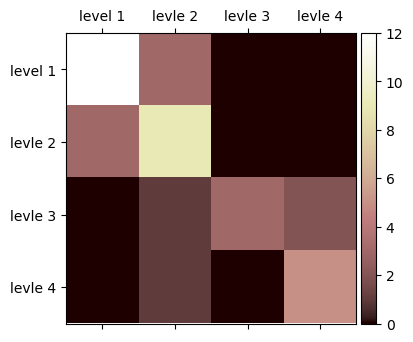
\includegraphics[width=\linewidth]{fig/conf_mx.png} 
	\caption{Confusion Matrix of XGBoost Result} 
	\label{fig:conf_mx} 
	% \ref{bear}
\end{figure}

In the normalised confusion matrix (\autoref{fig:norm_conf_mx}), it is clear that the darker square of level 4 is caused by the smaller 
data size of the class. The model is actually performing well even on smaller data size classes. That is why 
the macro-f1 is larger than micro-f1.\\[5pt]
\begin{figure}
	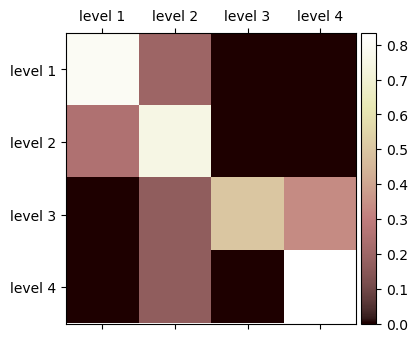
\includegraphics[width=\linewidth]{fig/norm_conf_mx.png} 
	\caption{Confusion Matrix of XGBoost Result} 
	\label{fig:norm_conf_mx} 
	% \ref{bear}
\end{figure}

From the feature importance table, it can be concluded that the severity of covid is more related 
to the human development index. The human development index is a score on the quality of living in the 
country including average life expectanvy, GDP, education opportunity, etc. The number of people fully 
vaccinated, the population composition or the diabetes prevalence do not play the most important role 
in the total cases as expected.   
%----------------------------------------------------------------------------------------
%	BIBLIOGRAPHY
%----------------------------------------------------------------------------------------

\printbibliography[title={Bibliography}] % Print the bibliography, section title in curly brackets

%----------------------------------------------------------------------------------------

\end{document}
